% !TEX root = ../YourName-Dissertation.tex

\chapter{Questions on the  local level}
This chapter talks about the reaction of subnational governments in the interaction with central government.The most frequently investigated question is the effect of IGT, A bunch of scholars devote time and energy to analyze and evaluate the impact of intergovernmental transfers. I summarize the literature into three categories. The first category focus on the impact on local governments' spending behavior. Under the local governments' spending behavior, two directions are highly documented. First direction concentrate on the effect of intergovernmental transfer on overall spending amounts of subnational government,such as the investigation on flypaper effect. Another direction investigate the micro-segments of the local governments' spending preference. The second category talks about the impact on local governments' revenue collection behavior, such as the investigation on local governments' tax effort, debt expansion tendency and issue and soft budget constrain behavior. The third category is about the effect of intergovernmental transfer across jurisdictions, such as the role of intergovernmental transfer in equalization. This chapter gives an overview on the most innovative literature and introduced the game theory tool under asymmetric setting to generate a theoretical model. The investigation directions can be summarized as Figure \ref*{Figure 3.1}.



\begin{figure}[H]
    \centering
    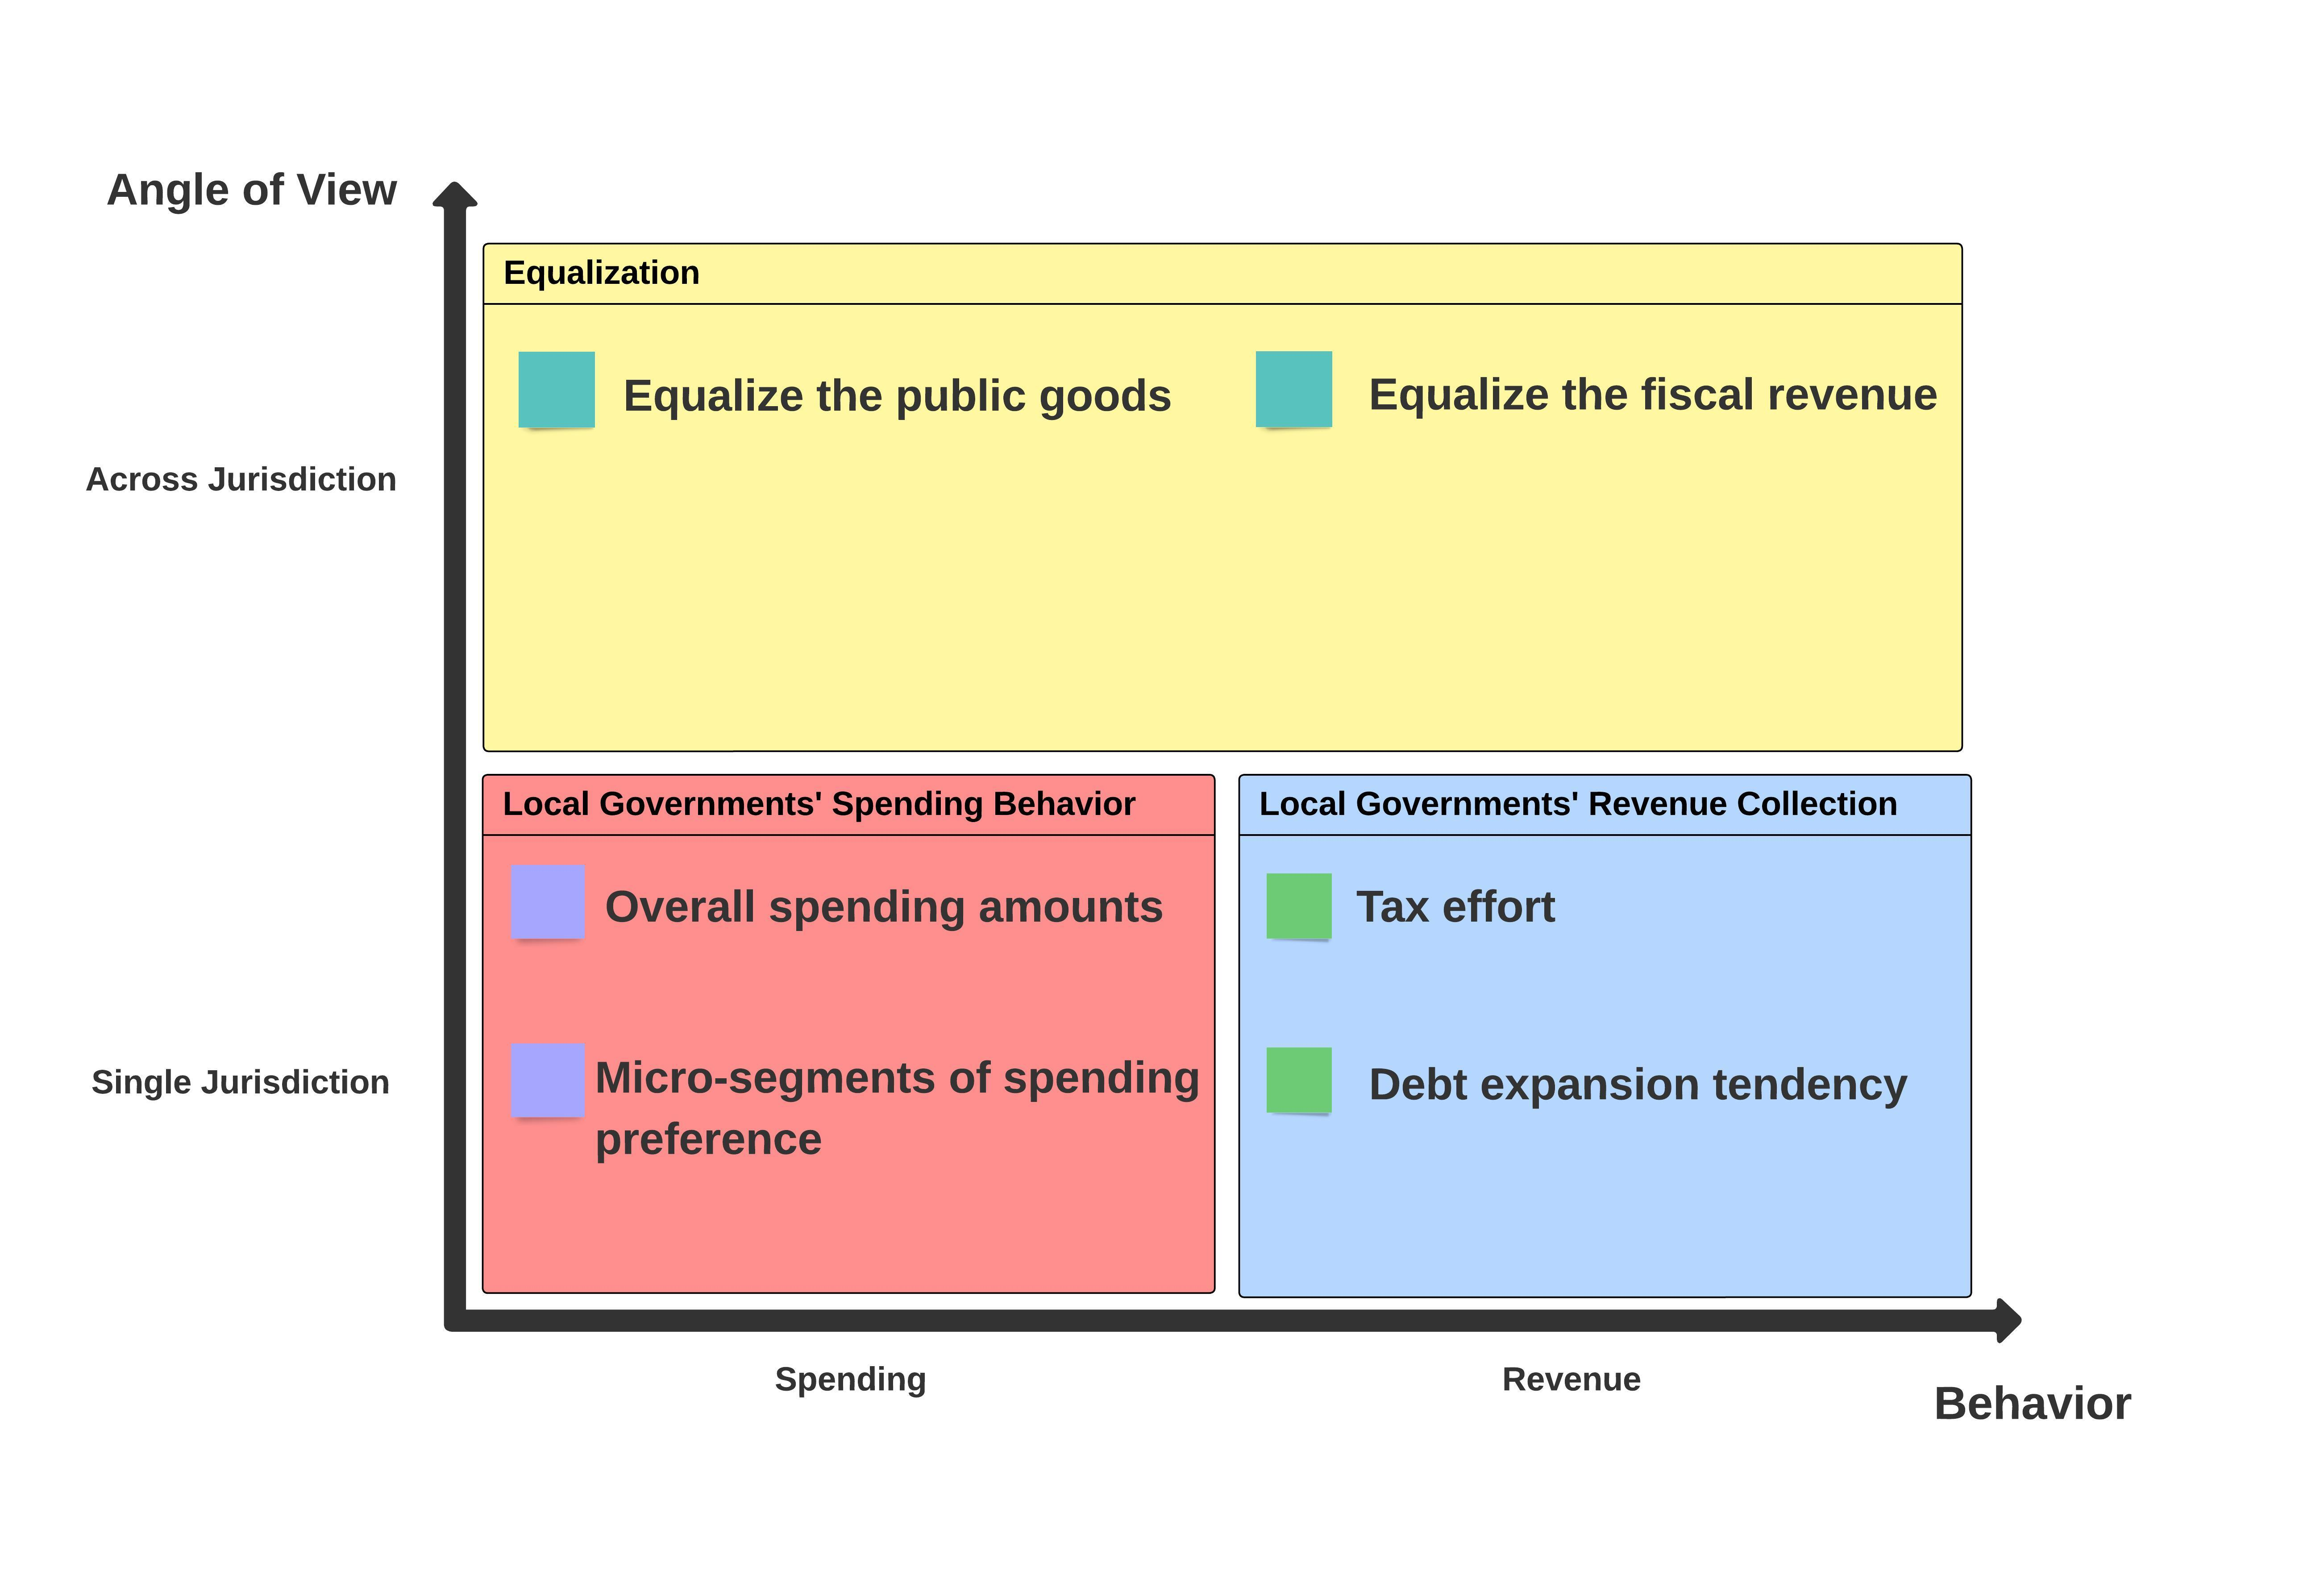
\includegraphics[scale=0.4]{Chapter-3/Figures/Effect of Intergovernmental Transfer.jpeg}
    \caption{Effect of Intergovernmental Transfer
        \texttt{} }
    \label{Figure 3.1}
\end{figure}




\section{Effect of IGT on Local Governments' Spending}

\subsection{Effect of IGT on Local Governments' Total Spending Amounts}

One intuitive philosophy is called "fungibility" \cite{pack1993foreign}, which means the intergovernmental transfer received by local government would substitute the local government's revenue. recipients assimilate dederal funds into general revenue and reduce the spending on public goods through a reduction of local taxes within the jurisdiction. However, supportive empirical evidence are quite limited. On the contrary, evidence on flypaper effect is widespread everywhere.

The fly paper effect is the most influential phenomenon during the vertical transfer from government in the fiscal federalism literature is  \cite{hines1995anomalies,gamkhar2007impact}. According to Bradford and Oates’s model, a lump sum grant from federal to state or local should be equivalent to the individual revenue increase within the jurisdiction in terms of the effect to stimulate the public expenditure \cite{bradford1971analysis}. The result conclusion is latterly known as equivalence theorem. Two assumptions play fundamental role in equivalence theorem. One is median voter theorem, another one is that federal, state and local government collect tax through lump sum tax. Under this theorem, money is money. However, the empirical evidence doesn’t support this theorem. More specifically, some researchers find that 1 dollar increase in personal increase would increase public expenditure by 0.02 to 0.05 dollar, while 1 dollar increase of intergovernmental transfer would trigger an increase of 0.25 to even 1 dollar in public expenditure \cite{bailey1998flypaper,dollery1996empirical,gamkhar2007impact}. This effect is known as flypaper effect. According to Inman's statistics, over 3,500 research papers investigate the flypaper effect both theoretically and empirically \cite{inman2008flypaper}.

In this section, I’m summarizing how scholars in different stages explain the flypaper effect. The understanding of flypaper effect went through a incremental progress, though may not be chronologically. This progress can be identified as three phrases. . In the first stage, the conventional analysis, scholars believe the matching grants have both price effect and income effects while the non-matching grants is analogous to the lump-sum subsidy, which means only income effects exists. In second stage, some scholars start to realize that non-matching grants has price effects as well, but that’s due to the impact of fiscal federalism setting and fiscal illusion. Federal government collecting revenue then redistributing to state and local generates fiscal illusion since this process is too complicated for consumers to perceive. In third stage, scholars start to realize the effect of distortionary tax that collect by grants recipient. The distortionary tax policy together with the low administrative efficiency in state and local leads to a higher marginal cost of the tax collection. Hence no matter the grants is matching or non-matching, the state or local government trend to use the grants rather than the tax revenue to cover the expenditure.

I set up a theoretical model and introduced the asymmetric setting into the model to explain all the local governments' reactions mentioned above. Started from a very simple Ramsey model and generalize it to more complicated scenarios.

\textbf{Benchmark model}

The Benchmark model is similar to Carlos and Guillermo's \cite{vegh2016unsticking} benchmark model with small modification.

To make the benchmark model as straight forward as possible while capture the IGT mechanism. I assume that:

\begin{enumerate}
    \item Economy is static.
    \item Only one local government and representative citizen in this economy.
    \item Two kinds of goods in the economy which are public good $G$ \label{G} and private good $X$.\label{X}
    \item Resident spend all there income $y$, which is given, on either private goods $X$ or tax $\tau$.\label{y}
    \item The tax is lump-sum tax with no dissertation.
    \item Source of government revenue: tax $\tau$ and transfer $f$.\label{f}
    \item Type of transfer: Nonmatching grants,like lump-sum subsidy.
\end{enumerate}

The representative citizen's budget constraint is:
\begin{equation}
    y=X+\tau \label{bmrc budgetc}
\end{equation}
The local government's budget constraint is:
\begin{equation}
    f+\tau=G \label{bmlg budgetc}
\end{equation}
Combine equation \ref{bmrc budgetc} and \ref{bmlg budgetc}, I get a budget constraint for the economy:
\begin{equation}
    y+f=X+G \label{bmecoconstrain}
\end{equation}
The utility for representative resident comes from the utility of $X$ and $G$. I assume the utility function is the Cobb-Douglas form thus it's a concave utility:
\begin{equation}
    U(X,G)=AX^{\alpha}G^{1-\alpha} , 0<\alpha<1 \label{bmrcutility}
\end{equation}
For the representative resident, the problem is to choose proper level of $X$ to maximize the utility in equation \ref{bmrcutility} subject to equation \ref{bmrc budgetc}. The Lagrangian equation can be set up as:
\begin{equation}
    L(X)=AX^{\alpha}G^{1-\alpha}+\lambda_{rc}(y-X-\tau)  \label{bmrclagrangian}
\end{equation}
Solving the equation \ref{bmrclagrangian} will get first order condition(foc):
\begin{equation}
    \alpha A\left(\frac{X}{G}\right)^{\alpha-1}=\lambda_{r c} \label{lamdarc}
\end{equation}
\begin{equation}
    y=X+\tau \label{rcfoc}
\end{equation}
To solve the Ramsey problem, the Ramsey planner needs to decide the level of $X,G$ to maximize the utility subject to equation \ref{bmecoconstrain} and equation \ref{bmlg budgetc}. The Lagrangian can be set as:
\begin{equation}
    L(X,G)=AX^{\alpha}G^{1-\alpha}+\lambda_{e}(y+f-X-G)+\lambda_{lg}(f+\tau-G)  \label{bmeclagrangian}
\end{equation}
Solving the equation \ref{bmeclagrangian} will generate:
\begin{equation}
    \alpha A\left(\frac{X}{G}\right)^{\alpha-1}=\lambda_e+\lambda_{l g}
    \label{foc on X}
\end{equation}
\begin{equation}
    (1- \alpha) A\left(\frac{X}{G}\right)^{\alpha}=\lambda_e+\lambda_{l g} \label{foc on G}
\end{equation}
\begin{equation}
    y+f=X+G \label{foc on lambdae}
\end{equation}
\begin{equation}
    f+\tau=G \label{foc on lambdalg}
\end{equation}

Combining equation \ref{foc on X}, \ref{foc on G}, \ref{foc on lambdae} will generate:
\begin{equation}
    (1-\alpha)y+(1-\alpha)f=G \label{bmresult}
\end{equation}
The flypaper effect definition can be mathematically expressed as $\frac{d G}{d f}-\frac{d G}{d y}$. Given equation \ref{bmresult}, the flypaper effect $fe=0$, which means, under this setting, theoretically there should be no flypaper effect.
\subsubsection{Phrase One}
Except for the introduction of intergovernmental transfer in \ref*{chapter1:Introduction}, One important concern about IGT in economic analysis is the matching mechanism. For matching grants, federal governments will reimburse a specific ratio for each 1 dollar of state and local expenditure. Based on whether federal government set a cap on the matching grants, matching grants can be divided into open-ended matching grants and closed-ended grants.

\textbf{Model with matching grants}

I loosen the last assumption in the benchmark model, now the intergovernmental transfer is 100\% matching grants which is expressed as $f_m$. Suppose the matching ratio is $m$ and $0<m<1$  \label{mr}.Thus the new budget constraint for local government is:
\begin{equation}
    \left\{\begin{array}{l} \label{mlgbudgetc}
        f_m+\tau=G \\
        f_m=m G
    \end{array}\right.
\end{equation}
And the budget constraint for the whole economy is:
\begin{equation}
    \left\{\begin{array}{l} \label{mebudgetc}
        y+f_m=X+G_M \\
        f_m=m G
    \end{array}\right.
\end{equation}
Thus the Ramsey problem is to choose proper level of $X$ and $G$ to maximize the utility subject to equation \ref{mebudgetc} and equation \ref{mlgbudgetc}.
So the new Lagrangian can be listed as:

\begin{equation} \label{mlagrangian}
    L(X,G)=AX^{\alpha}G^{1-\alpha}+\lambda_{e}(y+f_m-X-G)+\lambda_{lg}(f+\tau-G)
\end{equation}

Solving the equation \ref{mlagrangian}, I get foc conditions:
\begin{equation} \label{mfocs}
    \left\{\begin{array}{l}\alpha A \frac{X^{\alpha-1}}{G^{\alpha-1}}=\lambda_e+\lambda_{l g} \\ (1-\alpha) \frac{X^\alpha}{G^\alpha}=\lambda_e+\lambda_{l g} \\ y=X+(1-m) G\end{array}\right.
\end{equation}

By letting focs in equation \ref{mfocs} equals to zero, I get following equations:
\begin{equation} \label{myxandg}
    y=\frac{(1-\alpha)(1-m)+1}{1-\alpha} G
\end{equation}

thus the flypaper effect is calculated as $fe=\frac{d G}{d f_m}-\frac{d G}{d y}$
which equals to:
\begin{equation} \label{mfe}
    \frac{d G}{d f_m}-\frac{d G}{d y}=\frac{2 m \alpha-2 m-\alpha+2}{m[(1-\alpha)(1-m)+1]}
\end{equation}

\begin{figure}[H]
    \centering
    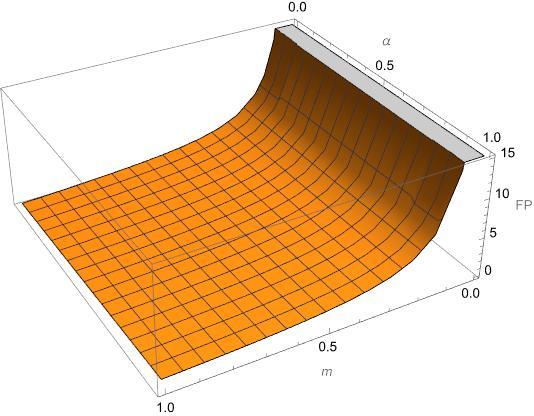
\includegraphics[scale=0.7]{Chapter-3/Figures/matchfp.jpg}
    \caption[Flypaper Effect with Matching Grants]{Flypaper Effect with Matching Grants
        \texttt{} }
    \label{Figure 3.2}
\end{figure}
Equation \ref*{mfe} could be proved to be greater than zero, which means for matching grants, the marginal contribution on public spending is higher than the marginal contribution of private income increase.\footnote[1]{The proof process is supplied in Appendix C}


\begin{figure}[H]
    \centering
    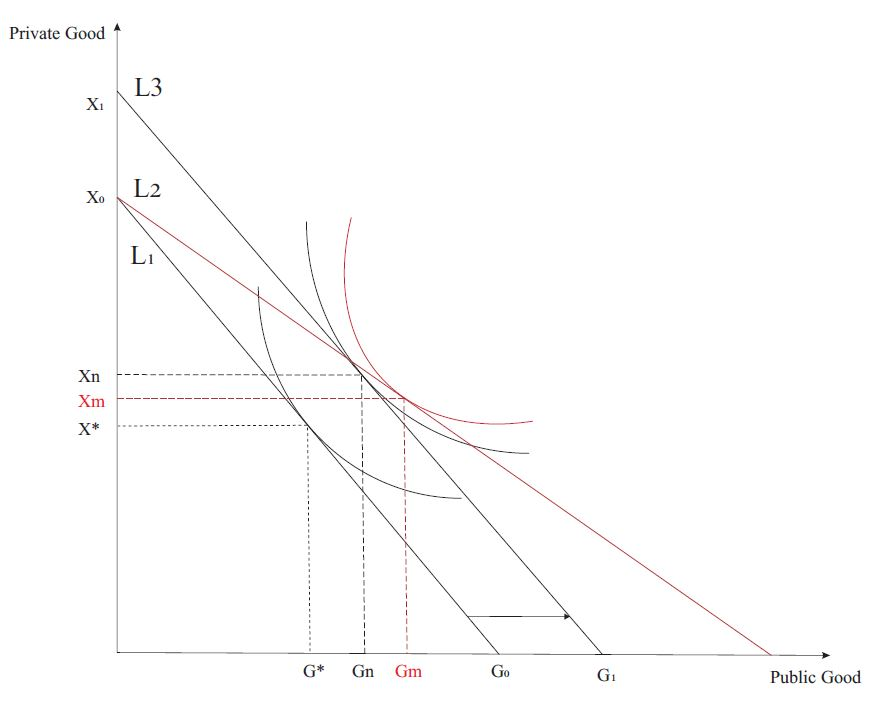
\includegraphics[scale=0.4]{Chapter-3/Figures/mfyeffect.jpg}
    \caption[Income Effect and Price Effect of Matching and Non-matching Grants]{Income Effect and Price Effect of Matching and Non-matching Grants
        \texttt{} }
    \label{Figure 3.3}
\end{figure}

As is shown in figure \ref{Figure 3.3}, the two parallel lines $L1$ and $L3$ are budget constraint of the economy before and after the non-matching grants and $L3$ is the budget constraint with matching grants which is the red line. The difference between $G_m$ and $G*$ is the combination of price effect and income effect of matching grants.

The matching grants model explains why scholars in first stage explain the fly paper effect due to misspecification or omitted variable. Misspecification means researchers may mix up matching grants with lump-sum grants. \cite{lankford1987note,henderson1968local}. Matching grants lower down the marginal price of public services, thus the mix-up will generate price effect and lead to more public goods spending \cite{gramlich1997state}. Some scholars attribute fly paper effects to omitted variables or pre-selection issue. Knight \cite{knight2002endogenous} designed a two-level bargaining model to prove that, federal government spread IGT to states and local governments with higher propensity to spend, so the flypaper effect is not a result of IGT. Former observations and investigations has endogenous issue. He also did an empirical test in which he designed an instrument variable to control the endogenous problem. He concludes that once we filter out the pre-selection issue, the flypaper effect is not obvious, at least for the data he collected about interstate highway programs. To summarize, the understanding under this view is that the flypaper effect doesn’t actually exist, it's just some kind of misspecification.

\subsubsection{Phrase two}

In stage two, scholars start to realize that lump-sum grants also have price effect, which is a huge step. In stage one, scholars recognized the price effect of matching grants, however they don’t think that’s enough to explain the huge gap in flypaper effect. If non-matching grants also have price effect, then it may be enough to explain. But in this stage, scholars claims that the price effect of non-matching grants exists because of the fiscal illusion. McCulloch \cite{mcculloch1845treatise} argues that taxpayers misperceived  the costs of governmental activity, which latterly be summarized as fiscal illusions.The theory of fiscal illusion was first developed by the Italian economist Amilcare Puviani in his 1903 book \textit{Teoria della illusione finanziaria} \cite{puviani1903teoria}. Wagner \cite{wagner1976revenue} firstly introduced this concept in America and pointed out the effect of fiscal illusion on local governments' spending. Oates and Borge notice the price effect of non-matching grants and try to use fiscal illusion to explain the price effect \cite{oates1979lump,borge1995lump}. The lower-estimated public good price generates a even flatter slope of the budget constraint compared to the $L3$ in figure \ref{Figure 3.3}.

Why fiscal illusion exists? Most explanation lies in the institutional setting and administrative transparency.The fiscal federalism setting is too complicated for residents to perceive. For administrative explanation, the administration process is not transparent enough for residents to understand every step. Hence, residents fail to recognize that the intergovernmental grants are collected from their income as well. Turnbull concludes in his empirical research that imperfect information generates broader fiscal illusion based on the municipal data \cite{turnbull1998overspending}. Besides, the budget-maximization intention of bureaucratic system are supported by both empirical evidence and theoretical inference \cite{mueller2003public,brennan1977towards}. This tendency is referred as "Leviathan government" by some scholars, which means governments seek to maximize their budget rather than maximize residents' utility \cite{quigley1986budget}. Budget-maximizing bureaucrat combined with the lower perceived price of the public goods price leads to a greater expenditure on public goods.

\subsubsection{Phrase Three}

In stage three, scholar focus on the effect of the cost of tax collection within the jurisdiction. The cost of tax collection comes from two aspects, one is the distortionary tax. No distortion for recipient tax revenue collection is a strong assumption. In reality, state and local government’s tax change lead to an obvious distortion of the residents’ behavior. The most apparent case is that residents may want to spend less time on working and more time on leisure once they are not satisfied about the tax and public goods policy, or they just move to another jurisdiction which is also a cost for the tax increase.

Hamilton \cite{hamilton1986flypaper} firstly notices that the distortionary tax within jurisdiction leads to a curved budget constraint, not a straight line.

\begin{figure}[H]
    \centering
    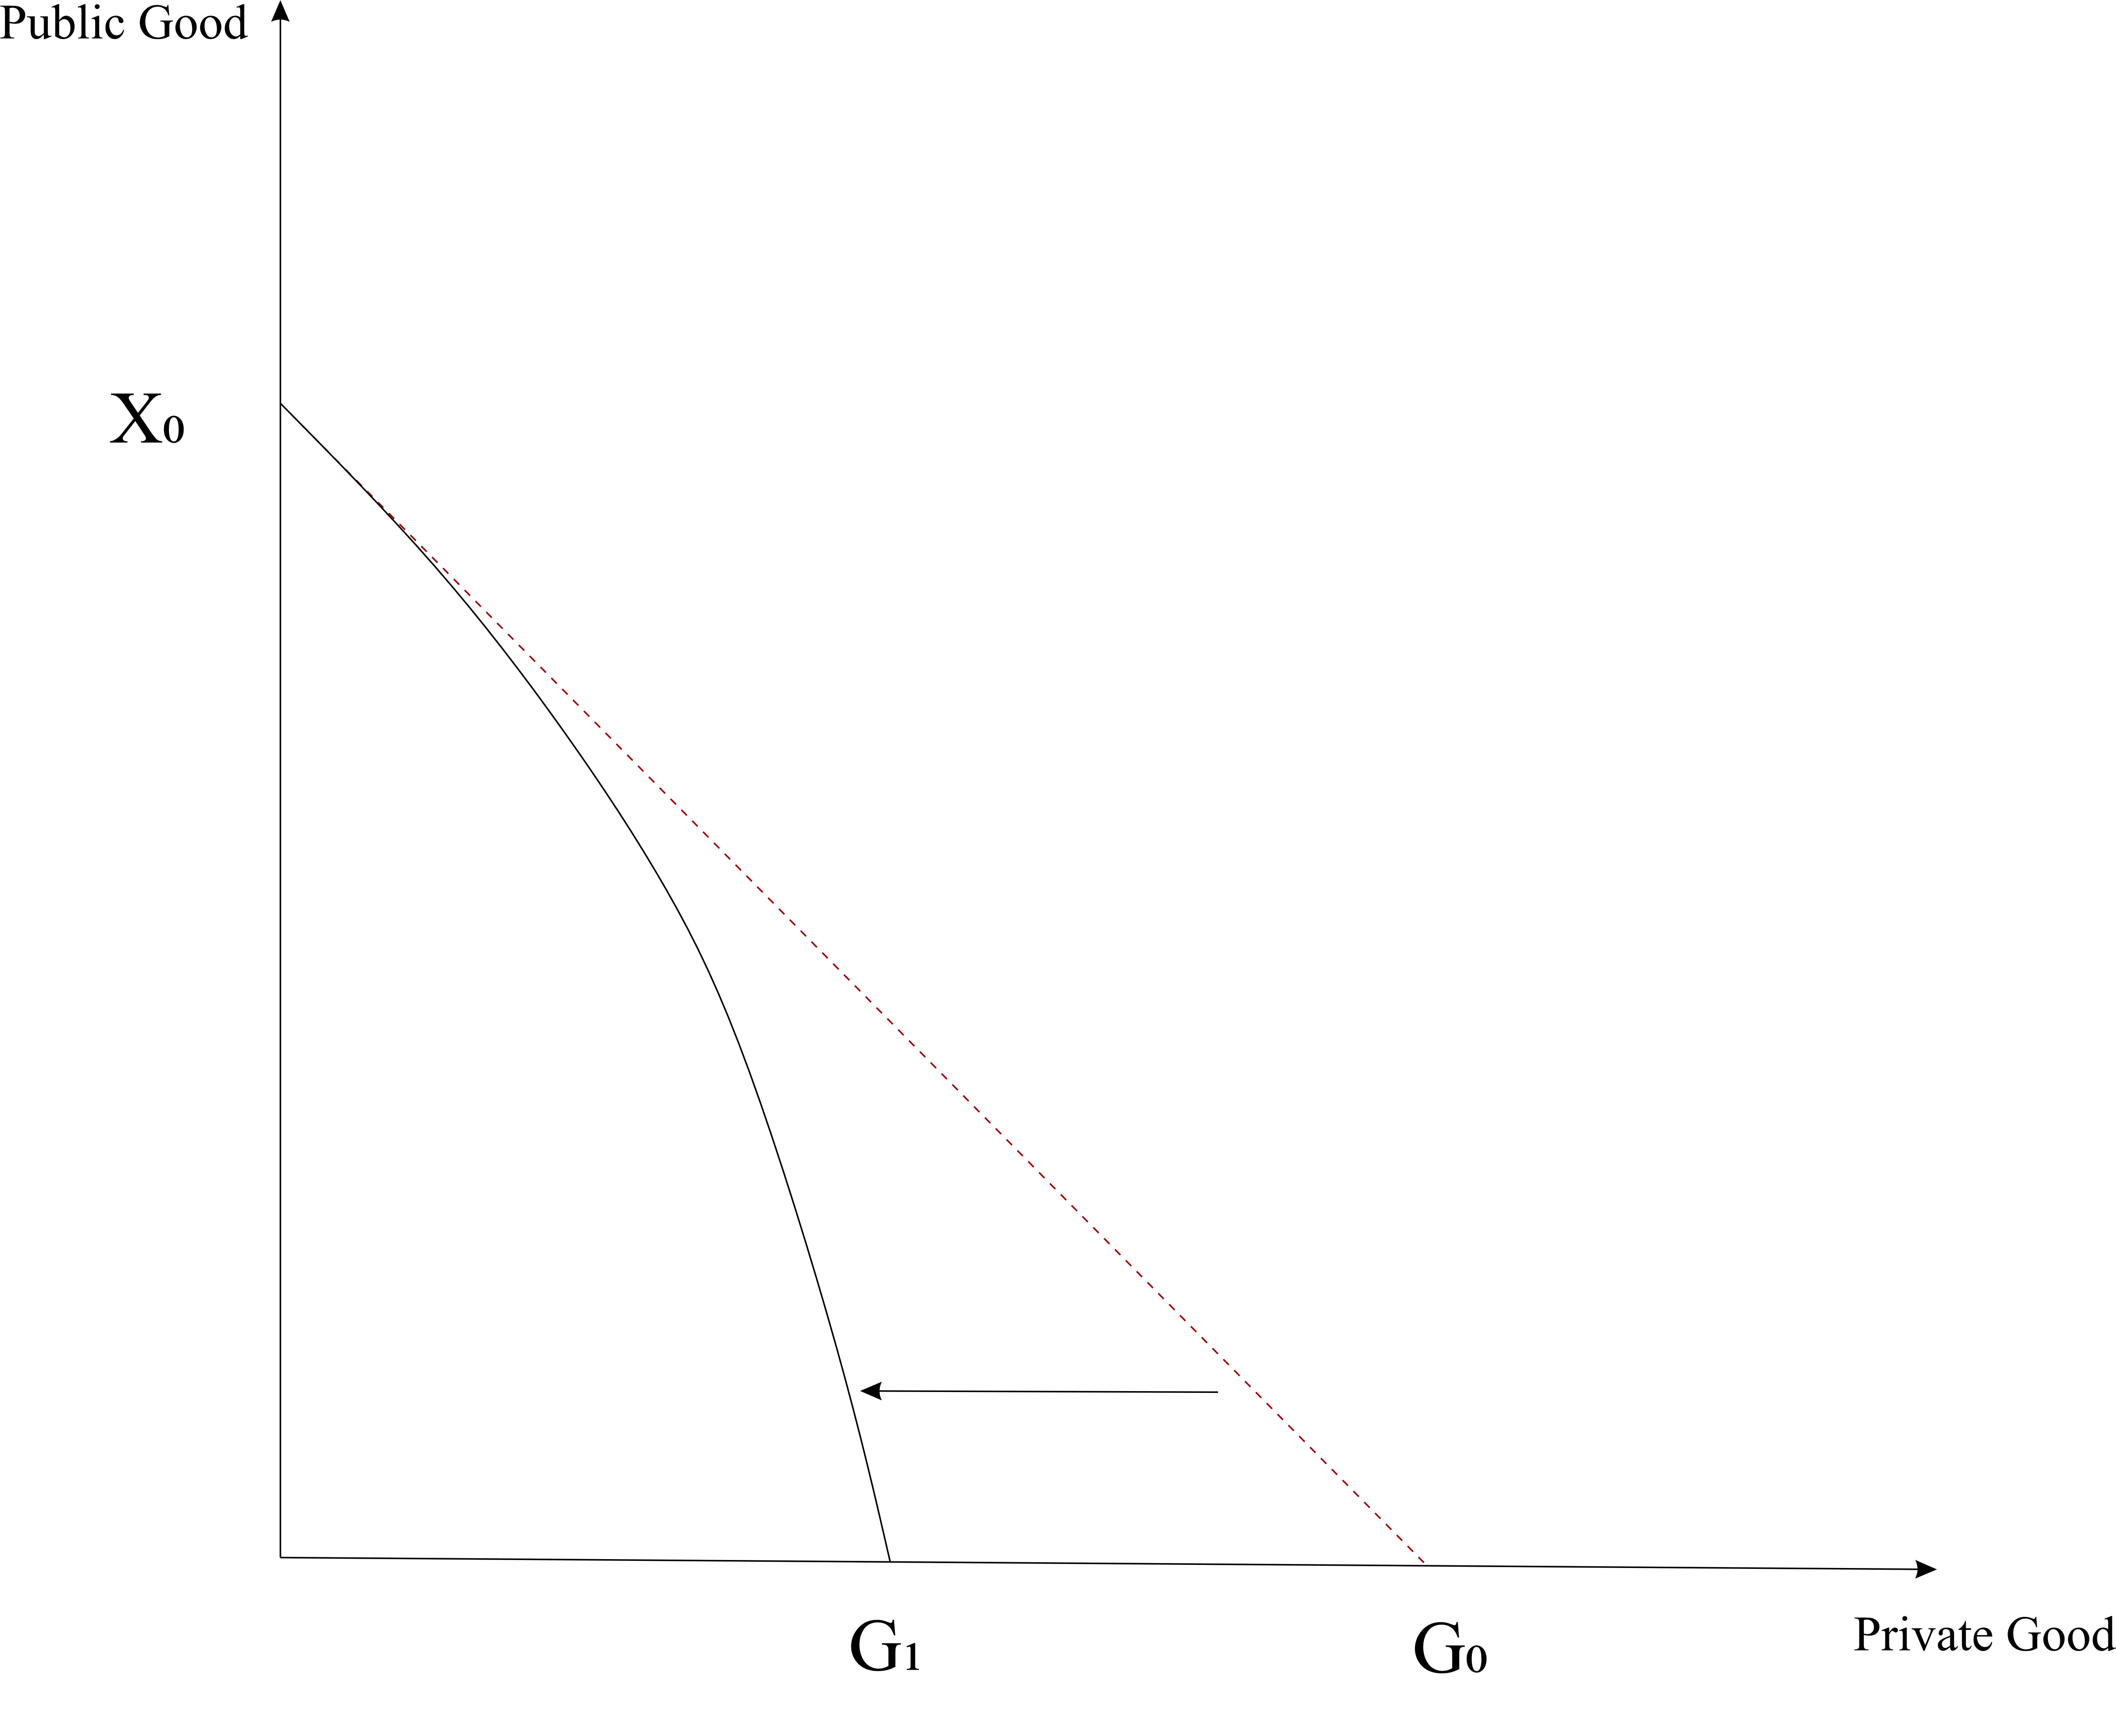
\includegraphics[scale=0.4]{Chapter-3/Figures/budget constrain distortion.jpg}
    \caption[Hamilton's Curved Budget Constraint]{Hamilton's Curved Budget Constrain
        \texttt{} }
    \label{Figure 3.4}
\end{figure}

However, Hamilton’s idea was not mainstream at that time. What’s more, he identifies the source of tax collecting cost is deadweight loss, ignores the administrative ability. In fact, the distortion is not the only source of cost. For example, the federal administrative institution is more effective and efficiency in collecting revenue based on the information or ability advantage.
Volden \cite{volden2007intergovernmental} designs a game theory model to simulate the interaction of federal government and lower-level governments, he implies that the different cost for federal and state governments to collect revenue partly explains the flypaper effect. Dahlby and Ferede \cite{dahlby2016stimulative} states that the price effect of non-matching grants exists even with no fiscal illusion. Vegh and Vuletin \cite{vegh2016unsticking} get similar conclusion as well. To summarize, the intuition of these research is straight forward: the collection of tax revenue is too costly for state and local government given the cost may come from both distortion and administrative inefficiency. The state and local government would more like to use “cheaper” resource, which is IGT. Hence, even non-matching grants or lump-sum grants have price effects.

Some horizontal government interaction explains this distortion as well, Brueckner \cite{brueckner2003strategic} develops a strategic model to analyze the state and local fiscal behavior, he concludes that the lower-level governments are quite sensitive to other competitors. This sensitivity may explain why state and local government don’t want tax increase revenue to cover the public goods. Other horizontal interaction theory such as yardstick competition or tax competition also explains the sensitivity.

I expand the benchmark model by introducing the distortion of tax collection into it.

\textbf{Ramsey Model with Distortionary Tax Collection}

To capture the distortion effect of the tax,I loosen the 3rd and 5th assumption of the benchmark model. I follow the setting by Carlos and Vuletin \cite{vegh2016unsticking} by adding a taxable private goods $X_t$ to differentiate with the non-taxable private goods $X_{nt}$ and capture the distortion effect of proportional tax. In reality, $X_{nt}$ could express any behavior that representative resident take to avoid the taxation, such as more time on leisure or
The assumption on taxation and representative resident's spending behavior are:
\begin{enumerate}
    \item Three kinds of goods in the economy which are public good $G$ and taxable private good $X_t$ and non-taxable private good $X_{nt}$.\label{Xt}
    \item Resident spend all there income $y$, which is given, on either taxable private goods $X_t$, non-taxable private goods $X_{nt}$ or tax.
    \item The tax is proportionary tax on $X_{t}$, with tax rate $\theta$.
\end{enumerate}

So the budget constrain for resident, local government and the whole economy could be separately list as:
\begin{equation} \label{distortionrct}
    y=X_t(1+\theta)+X_{n t}
\end{equation}
\begin{equation} \label{distortiongct}
    f+\theta X_t=G
\end{equation}
\begin{equation} \label{distortionect}
    y+f=x_t+x_{nt}+G
\end{equation}

Different from Carlos' setting who accept a more general setting on residents' and governments' utility, I set Cobb-Douglas form on utility to get a arithmetic solution. Unlike the benchmark model in Carlos' research, in which he set the linear utility, the Cobb-Douglas setting means the imperfect substitute between private and public goods, which is a more reasonable setting. The distribution on $X_t$, $X_{nt}$ and $G$ should maximize representative resident's utility and government's utility.
\begin{equation} \label{rclgutility}
    \left\{\begin{array}{l}U=A X^\alpha G^{1-\alpha} \\ X=B X_t^\beta X_{n t}^{1-\beta}\end{array}\right.
\end{equation}
Where X represent a composite private good.
For resident, they need to decide $X_t, X_{nt}$ to maximize $U$ subject to equation \ref{distortionrct}. For local government, the problem is to decide the distribute of $X$ and $G$ to maximize $U$, thus the Ramsey problem is to maximize both resident and local governments' utility, which is listed as equation \ref*{rclgutility} subject to equation \ref{distortionrct} and \ref{distortiongct}. For resident, the first order conditions on $X_t, X_{nt}, \lambda_{rc}$ can be listed as:
\begin{align}
    \begin{split}
        \frac{\partial U}{\partial X} \frac{\partial X}{\partial X_t}=(1+\theta) \lambda_{r c} \label{focxt}
    \end{split}                     \\
    \begin{split}
        \frac{\partial U}{\partial X} \frac{\partial X}{\partial X_{nt}}=\lambda_{r c} \label{focxnt}
    \end{split} \\
    \begin{split}
        y=X_t(1+\theta)+X_{nt} \label{foclabrc}
    \end{split}
\end{align}
Solving equation \ref{focxt}, \ref{focxnt} will generate the relationship between $X_t$ and $X_{nt}$ in equilibrium and the level of $\theta$:
\begin{align}
    \begin{split}
        X_{nt}=\frac{(1-\beta)(1+\theta)}{\beta}X_t \label{xtxnt}
    \end{split} \\
    \begin{split}
        \theta=\frac{\beta X_{n t}}{(1-\beta) X_t}-1 \label{theta}
    \end{split}
\end{align}

For local government and Ramsey Planner, they need to decide $G, X_t, X_{nt}$ subject to equation \ref*{distortiongct} and \ref*{distortionect}, the FOCs on $X_t, X_{nt}, G, \lambda_e, \lambda_{lg}$ are:
\begin{align}
    \begin{split}
        \frac{\partial U}{\partial X} \frac{\partial X}{\partial X_t}=\lambda_e+\lambda_{l g}
    \end{split}                                                       \\
    \begin{split}
        \frac{\partial U}{\partial X} \frac{\partial X}{\partial X_{nt}}=\lambda_e +\frac{\beta}{1-\beta} \lambda_{l g}
    \end{split} \\
    \begin{split}
        \frac{\partial U}{\partial G}=\lambda_e+\lambda_{l g}
    \end{split}                                                                                       \\
    \begin{split}
        y+f=x_t+x_{nt}+G
    \end{split}                                                                                                                            \\
    \begin{split}
        f+\theta X_t=G
    \end{split}
\end{align}
Follow the definition of $fe$ in equation \label{mfe}, the flypaper effect under distortionary taxation can be calculated as:

\begin{figure}[H]
    \centering
    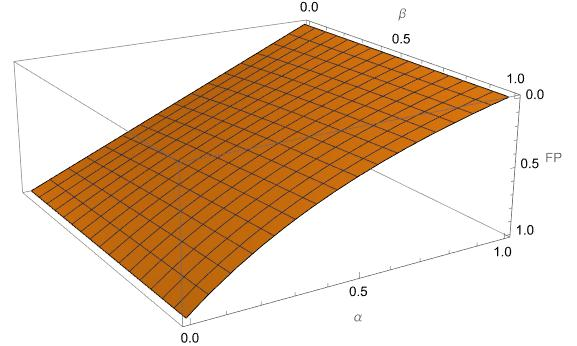
\includegraphics[scale=0.7]{Chapter-3/Figures/distorfp.jpg}
    \caption[Flypaper Effect under Distortionary Taxation]{Flypaper Effect under Distortionary Taxation
        \texttt{} }
    \label{Figure 3.5}
\end{figure}

\subsection{Effect of IGT on Local Governments' Spending Segments}
% The investigation on the spending preference is related with the investigation of local governments' tax effort.
Unlike the investigation on overall spending amounts, the understanding of the impact of intergovernmental transfer on micro-segments spending varies. The scholars focus not only on the matching mechanism, but also on restriction of the purpose when analyzing the impact on spending preference. To be more specific, general transfer (such as general revenue sharing in Table \ref{Table 1.1}) and transfer with special purpose (such as block grants and project categorical grants Table \ref{Table 1.1}) may cause different effect on local governments' spending preference. For one, some empirical evidence still implies the flypaper effect, which means the intergovernmental transfer stimulate local governments' spending in specific area. Feldstein notice the categorical grants in education field from Massachusetts state government to local governments lead to higher local governments' spending on education \cite{feldstein1975wealth}. Karnik and Lalvani \cite{karnik2008flypaper} incorporate the spatial effect into their model when analyzing the data from Maharashtra in India. They found that an increase in intergovernmental grants results in the urban local governments spending more on specific expenditure categories than they would have from an equivalent increase in incomes.

Except for the flypaper effect, another widely discussed phenomenon on categorical governments spending preference is fungibility \cite{pack1993foreign}. The fungibility of intergovernmental transfer means the intergovernmental transfer received by local government would substitute the local government's revenue. Local government may alter the spending structure based on their own preference rather than follow the strings attached on the intergovernmental transfer. One evidence is that subnational governments in Latin America prefer to use the money to cover administrative expense \cite{stein1999fiscal}. Once the transfer with specific purpose received by the local governments, the own-generated revenue got crowded out and flow into the preferred area. Another supportive evidence is founded in China. Researchers divides all public spending categories into either productive area, such as the input on infrastructure, or public service area, such as public medicare or education. Empirical evidence implies that local government prefer to crowd out the revenue which should have been invested in public service area and move them to productive spending once they received the intergovernmental transfer even if the transfer is restricted to specific category \cite{yinheng2011,fuyong2010}.

One potential issue is that most of the investigation on spending preference focus on the spending sector independently, which is the lower left part of figure \ref{Figure 3.1}. I think the spending preference could not be investigated in isolation. For example,  Thus I incorporate the revenue behavior into the model to evaluate the spending behavior after the introduction of Section 3.2.

Another issue is that most of the investigation mentioned above are empirical evidence without a general framework to explain it theoretically, thus I'll introduce the asymmetric setting into the model to explain the spending preference based on the theoretical setting I generated to explain the flypaper effect.

\section{Effect of IGT on Local Governments' Revenue Collection Behavior}

Intuitively, the general transfer should have a substitute effect on local governments' revenue collection effort, which is referred as tax fungibility effect. In some literature, it's called crowding effect on tax effort and it's supported by bunch of scholars \cite{inman1988federal,peterson1997decentralization,litvack1998rethinking}. Based on this theoretical inference, empirical evidence are founded in both developed and developing countries. Nicholson \cite{nicholson2008fiscal} found the fungibility effect of intergovernmental transfer on tax effort on state level in Germany and America separately. Baretti \cite{2002A}, Aragon and Gayoso \cite{aragon2005intergovernmental}, Panda \cite{panda2009central}, Mogues \cite{mogues2012external} and Bravo \cite{bravo2013income} found similar evidence in developing countries such as Peru, India, Ghana and Chile. However, the fungibility effect of categorical grants are seldom investigated. To summary, the fungibility of intergovernmental transfer on tax revenue makes governments lower down their effort to collect tax revenue once they got enough funds from transfer payments.

The fungibility effect seems natural when the range of study is constrained in one specific jurisdictions. Once multiple jurisdictions and horizontal competition are introduced into the consideration, one opposite impact also seems to be reasonable. Some theoretical research contend that the local jurisdictions should be motivated to lower the tax burden since they are facing the tax competition. The lower tax burden may attract capital, citizen or enterprise into the area, thus the local governments may actively give up the tax benefits they could have collected. In another word, the tax competition may encourage the local governments to expand the tax base rather than increase the tax effort. The revenue from intergovernmental transfer may neutralize this subjective intention, thus the tax effort would be positively affected. Bucovetsky and Smart \cite{2010The}, Buettner \cite{2006The} describe this guess in their analysis of fiscal equalization. Liu \cite{2011Intergovernmental}
found some empirical evidence in China. However, compared to the study on fungibility, the investigation on this effect are seldom systemically investigated in theoretical level, limited literature are empirical analysis.

To summarize the literature, there are two potential gaps. Firstly, like the literature on the effect of IGT on local governments' spending preference, the discussion is heavily concentrated on general transfer rather than categorical transfer, thus the effect of categorical transfer on tax revenue collection behavior are barely investigated. Brunt and Khdari \cite{2016The} did a research about the effect of categorical grants using the data collected in Morocco, unfortunately they do not get a clear conclusion. They ascribe the insignificant result to the political impact thus leave room for local governments to bargain. Secondly, limited literature focus on the theoretical base of the second effect, which may positively affect the tax effort. Thus I designed a asymmetric setting through a dynamic game with incomplete information to simulate the  behavior of central and local governments. And I combine the game theory analysis result with the prototypical benchmark model in section 3.1.1 to connect both spending side (lower left side of Figure \ref{Figure 3.1}) and revenue side (lower right side of Figure \ref{Figure 3.1}). This model could be helpful in understanding the central and local governments' behavior on the theoretical level. Finally in Chapter 4, I'll empirically investigate my theoretical inference.

\section{A Dynamic Game with Incomplete Information for Central and Local Governments}


